\subsection{BÀI TẬP TRẮC NGHIỆM}
% \ind{PHẦN I.} \inden{Câu trắc nghiệm nhiều phương án lựa chọn. Học sinh trả lời từ câu 1 đến câu 12. Mỗi câu hỏi học sinh chỉ chọn một phương án.}\\
\TN
\setcounter{ex}{0}
\Opensolutionfile{ans}[ans/1D5-B3-1]
\begin{ex}%Câu 1%[1D3N3-2]
	Hàm số $f$ liên tục tại  $x_0=1$. Đồ thị của $f$ có thể là hình nào dưới đây?
	\choice
	{\True 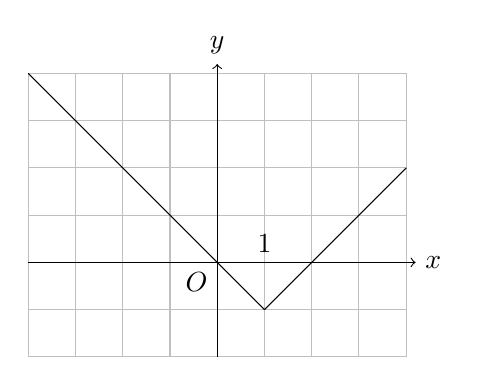
\begin{tikzpicture}[scale=0.6]
			\draw[thin,color=gray!50] (-4,-2) grid (4,4);
			\draw[->] (-4,0) -- (4.2,0) node[right] {$x$};
			\draw[->] (0,-2) -- (0,4.2) node[above] {$y$};
			\draw[domain=-4:1] plot (\x,-\x);
			\draw[domain=1:4] plot (\x,\x-2);
			\draw (0,0) node[below left]{$O$};
			\draw (1,0) node[above]{$1$};
	\end{tikzpicture}}
	{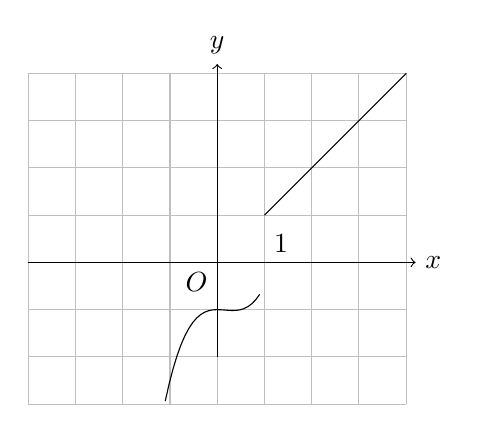
\begin{tikzpicture}[scale=0.6]
			\draw[thin,color=gray!50] (-4,-3) grid (4,4);
			\draw[->] (-4,0) -- (4.2,0) node[right] {$x$};
			\draw[->] (0,-2) -- (0,4.2) node[above] {$y$};
			\draw[domain=-1.1:0.9] plot (\x,{(\x)^3-0.5*(\x)^2-1});
			\draw[domain=1:4] plot (\x,\x);
			\draw (0,0) node[below left]{$O$};
			\draw (1,0) node[above right]{$1$};
	\end{tikzpicture}}
	{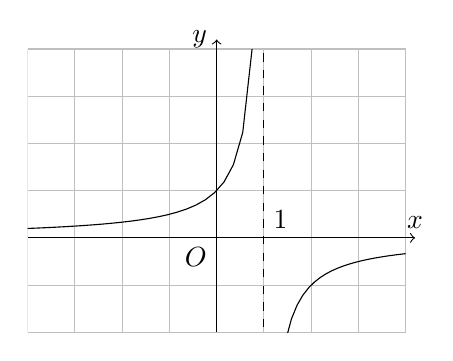
\begin{tikzpicture}[scale=0.6]
			\clip (-4,-2) rectangle (4.4,4.45);
			\draw[thin,color=gray!50] (-4,-2) grid (4,4);
			\draw[->] (-4,0) -- (4.2,0) node[above] {$x$};
			\draw[->] (0,-2) -- (0,4.2) node[left] {$y$};
			\draw[domain=-4:0.75] plot (\x,{(-1)/((\x)-1)});
			\draw[domain=1.1:4] plot (\x,{(-1)/((\x)-1)});
			\draw [dashed] (1,-4)--(1,4);
			\draw (0,0) node[below left]{$O$};
			\draw (1,0) node[above right]{$1$};
	\end{tikzpicture}}
	{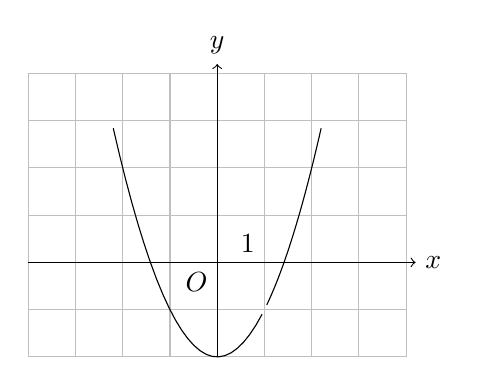
\begin{tikzpicture}[scale=0.6]
			\draw[thin,color=gray!50] (-4,-2) grid (4,4);
			\draw[->] (-4,0) -- (4.2,0) node[right] {$x$};
			\draw[->] (0,-2) -- (0,4.2) node[above] {$y$};
			\draw[domain=-2.2:0.95] plot (\x,{(\x)^2-2});
			\draw[domain=1.05:2.2] plot (\x,{(\x)^2-2});
			\draw (0,0) node[below left]{$O$};
			\draw (1,0) node[above left]{$1$};
	\end{tikzpicture}}
	\loigiai{
		Hàm số có đồ thị như sau liên tục tại $x_0=1$.
		\begin{center}
			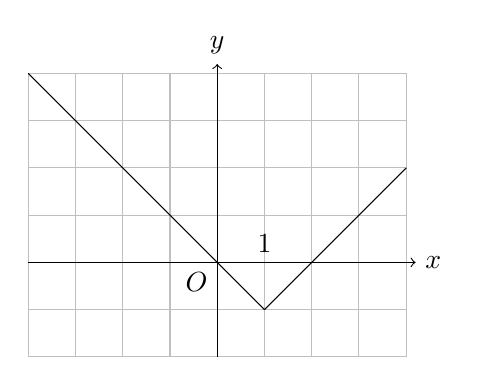
\begin{tikzpicture}[scale=0.6]
				\draw[thin,color=gray!50] (-4,-2) grid (4,4);
				\draw[->] (-4,0) -- (4.2,0) node[right] {$x$};
				\draw[->] (0,-2) -- (0,4.2) node[above] {$y$};
				\draw[domain=-4:1] plot (\x,-\x);
				\draw[domain=1:4] plot (\x,\x-2);
				\draw (0,0) node[below left]{$O$};
				\draw (1,0) node[above]{$1$};
			\end{tikzpicture}
		\end{center}
	}
\end{ex}	
\begin{ex}%Câu 2%[1D3N3-1]
	Cho hàm số $y=f( x )$ liên tục trên $(a;b)$. Điều kiện cần và đủ để hàm số liên tục trên $\left[a;b \right]$ là
	\choice
	{$\lim\limits_{x\to a^+}f(x)=f(a)$ và $\underset{x\to b^+}{\mathop{\lim }}\,f(x)=f(b)$}
	{\True $\lim\limits_{x\to a^+}f(x)=f(a)$ và $\lim\limits_{x\to b^-}f(x)=f(b)$}
	{$\lim\limits_{x\to a^-}f(x)=f(a)$ và $\lim\limits_{x\to b^+}f(x)=f(b)$}
	{$\lim\limits_{x\to a^-}f(x)=f(a)$ và $\lim\limits_{x\to b^-}f(x)=f(b)$}
	\loigiai{
		Hàm số $y=f( x )$ liên tục trên $(a;b)$. Điều kiện cần và đủ để hàm số liên tục trên $\left[ a;b \right]$ là $\lim\limits_{x\to a^+}f(x)=f(a)$ và $\lim\limits_{x\to b^-}f(x)=f(b)$.
	}
\end{ex}
\begin{ex}%Câu 3%[1D3N3-3]
	Hàm số $y=\dfrac{1}{x(x^2-9)}$ liên tục tại điểm nào dưới đây?
	\choice
	{$0$}
	{$3$}
	{$-3$}
	{\True $1$}
	\loigiai{
		Điều kiện xác định: $x(x^2-9)\ne 0\Leftrightarrow \heva{& x\ne 0 \\& x\ne \pm 3.}$\\
		Suy ra hàm số liên tục trên các khoảng $( -\infty;-3 )$, $( -3;0 )$, $( 0;3 )$, $( 3;+\infty  )$.\\
		Vậy hàm số liên tục tại $x=1$.	
	}
\end{ex}
\begin{ex}%Câu 4%[1D3N3-3]
	Hàm số $y=\dfrac{1}{4x-4}$ gián đoạn tại điểm nào dưới đây?
	\choice
	{\True $x=1$}
	{$x=0$}
	{$x=2$}
	{$x=-1$}
	\loigiai{
		Tập xác định $\mathscr{D}=\mathbb{R}\backslash \left\{ 1 \right\}$, suy ra hàm số gián đoạn tại $x=1$.	
	}
\end{ex}
\begin{ex}%Câu 5%[1D3N3-4]
	Hàm số nào sau đây \textbf{không} liên tục trên tập số thực $\mathbb{R}$?
	\choice
	{\True $y=\dfrac{4}{x}+\dfrac{7}{9}$}
	{$y=4x+\dfrac{7}{9}$}
	{$y=\sin2x$}
	{$y=3x^2+\sqrt{5}$}
	\loigiai{
		Hàm số $y=\dfrac{4}{x}+\dfrac{7}{9}$ có tập xác định là $\mathbb{R}\setminus \left\{ 0 \right\}$.	
	}
\end{ex}
\begin{ex}%Câu 6%[1D3N3-3]
	Hàm số nào sau đây \textbf{không} liên tục tại $x=2$?
	\choice
	{$y=\sin x$}
	{\True $y=\dfrac{x^2}{x-2}$}
	{$y=x^2-3x+2$}
	{$y=\sqrt{x+2}$}
	\loigiai{
		Ta thấy hàm số $y=\dfrac{x^2}{x-2}$ có tập xác định là $\mathscr{D}=\mathbb{R}\backslash \left\{ 2 \right\}$ nên hàm số không liên tục tại $x=2$.}
\end{ex}
\begin{ex}%Câu 7%[1D3N3-3]
	Hàm số $y=\dfrac{3}{x(x+1)(x+2)}$ liên tục tại điểm nào dưới đây?
	\choice
	{$x=-1$}
	{$x=-2$}
	{\True $x=3$}
	{$x=0$}
	\loigiai{
		Tập xác định của hàm số $y=\dfrac{3}{x( x+1 )( x+2 )}$ là $\mathscr{D}=\mathbb{R}\setminus\left\{ -2;-1;0 \right\}$.\\
		Vậy hàm số đã cho liên tục trên các khoảng xác định của nó.
		Suy ra hàm số liên tục tại điểm $x=3$.
	}
\end{ex}
\begin{ex}%Câu 8%[1D3H3-3]
	Cho hàm số $f(x)=\heva{
		& \dfrac{x^3+8}{4x+8}\; &\text{ khi } x\ne -2 \\ 
		& 3\; &\text{ khi } x=-2}$. Chọn khẳng định đúng trong các khẳng định sau?
	\choice
	{Hàm số $f( x )$ không liên tục trên tập $\mathbb{R}$}
	{Hàm số $f( x )$ có tập xác định là $\mathbb{R}\setminus \left\{ -2 \right\}$}
	{Hàm số $f( x )$ gián đoạn tại $x=2$}
	{\True Hàm số $f( x )$ liên tục tại $x=-2$}
	\loigiai{
		Tập xác định: $\mathscr{D}=\mathbb{R}$.\\
		Ta có $f(-2)=3$ và \\
		$\lim\limits_{x\to -2}f(x)=\lim\limits_{x\to -2}\dfrac{x^3+8}{4x+8}=\lim\limits_{x\to -2}\dfrac{(x+2)(x^2-2x+4)}{4( x+2 )}=\lim\limits_{x\to -2}\dfrac{x^2-2x+4}{4}=3$.\\
		Suy ra $\lim\limits_{x\to -2}f( x )=f( -2 )$ hay hàm số $f( x )$ liên tục tại $x=-2$.}
\end{ex}
\begin{ex}%Câu 9%[1D3H3-3]
	Số điểm gián đoạn của hàm số $f(x)=\dfrac{\sin x}{x^3+3x^2-2x-2}$ là
	\choice
	{$1$}
	{\True $3$}
	{$0$}
	{$2$}
	\loigiai{
		Ta có $x^3+3x^2-2x-2=0\Leftrightarrow \hoac{& x=1 \\ & x=-2-\sqrt{2} \\ 	& x=-2+\sqrt{2}}$\\
		nên hàm số liên tục trên $( -\infty ;-2-\sqrt{2} )$, $( -2-\sqrt{2};-2+\sqrt{2} )$, $( -2+\sqrt{2};1 )$ và $( 1;+\infty  )$.
		\begin{center}
			\begin{tikzpicture}
				\tkzTabInit[lgt=4,espcl=3]
				{$x$/0.7,$x^3+3x^2-2x-2$/0.7}
				{$-\infty$,$-2-\sqrt{2}$,$-2+\sqrt{2}$,$1$,$+\infty$}
				\tkzTabLine{ ,-,0,+,0,-,0,+, }
			\end{tikzpicture}
		\end{center}
		Ta có: $\lim\limits_{x\to ( -2-\sqrt{2} )^-}f( x )=-\infty $ vì 
		$\heva{&\lim\limits_{x\to ( -2-\sqrt{2} )^-}\sin ( x )\simeq 0,27\\
			& \lim\limits_{x\to ( -2-\sqrt{2} )^-}( x^3+3x^2-2x-2 )=0
			\text{ và } x^3+3x^2-2x-2<0.}$\\
		
		$\lim\limits_{x\to ( -2-\sqrt{2} )^+}f( x )=+\infty$ vì $\heva{&\lim\limits_{x\to ( -2-\sqrt{2} )^+}\sin ( x )\simeq 0,27\\ &\lim\limits_{x\to ( -2-\sqrt{2} )^+}(x^3+3x^2-2x-2 )=0	\text{ và } x^3+3x^2-2x-2>0.}$\\
		Suy ra: $\lim\limits_{x\to ( -2-\sqrt{2} )}f(x)$ không tồn tại nên hàm số bị gián đoạn tại $x_0=-2-\sqrt{2}$.		
	}
\end{ex}
\begin{ex}%Câu 10%[1D3H3-4]
	Trong các hàm số sau, hàm số nào liên tục trên $\mathbb{R}$?
	\choice
	{$f(x)=\cot 2x$}
	{\True $f(x)=\heva{
			&\dfrac{10-2x}{\sqrt{x+11}-4}\; &\text{ khi } x\ne 5 \\ 
			& -16\; &\text{ khi } x=5}$}
	{$f(x)=\heva{& 4x+3\; &\text{ khi } x<-2 \\ 
			& 3{{x}^{2}}-7\; &\text{ khi } x\ge -2}$}
	{$f(x)=\sqrt{2x-1}+\sqrt{1+5x}$}
	\loigiai{
		Hàm số $f(x)=\cot 2x$ và $f(x)=\sqrt{2x-1}+\sqrt{1+5x}$ có tập xác định không phải là $\mathbb{R}$.\\
		Hàm số $f(x)=\heva{& 4x+3\; &\text{ khi } x<-2 \\ 
			& 3{{x}^{2}}-7\; &\text{ khi} x\ge -2}$ không liên tục tại $x=-2$.\\
		Hàm số $f(x)=\heva{
			&\dfrac{10-2x}{\sqrt{x+11}-4}\; &\text{ khi } x\ne 5 \\ 
			& -16\; &\text{ khi } x=5}$ có\\
		$\lim\limits_{x\to 5}\dfrac{10-2x}{\sqrt{x+11}-4}=\lim\limits_{x\to 5}\dfrac{( 10-2x )( \sqrt{x+11}+4 )}{x+11-16}=\lim\limits_{x\to 5}\left[ -2( \sqrt{x+11}+4 ) \right]=-16$.		
	}
\end{ex}
\begin{ex}%Câu 11%[1D3H3-4]
	Cho bốn hàm số $f_1(x)=2x^3-3x+1$, $f_2(x)=\dfrac{3x+1}{x-2}$, $f_3(x)=\cos x+3$ và $f_4(x)=\tan x$. Hỏi có bao nhiêu hàm số liên tục trên tập $\mathbb{R}$?
	\choice
	{$1$}
	{\True $2$}
	{$3$}
	{$4$}
	\loigiai{
		\begin{itemize}
			\item  Ta có hai hàm số $f_2(x)=\dfrac{3x+1}{x-2}$ và $f_4(x)=\tan x$ có tập xác định không phải là tập $\mathbb{R}$ nên không liên tục trên tập $\mathbb{R}$.
			\item Cả hai hàm số $f_1(x)=2x^3-3x+1$ và $f_3(x)=\cos x+3$ đều có tập xác định là $\mathbb{R}$ đồng thời liên tục trên $\mathbb{R}$.
		\end{itemize}
	}
\end{ex}
\begin{ex}%Câu 12%[1D3H3-3]
	Cho $f(x)$, $g(x)$ là các hàm số liên tục tại $x=3$. Biết $f(3)=4$ và $\lim\limits_{x\to 3}\left[ 3f(x)-g(x) \right]=6$. Tính $g(3)$.
	\choice
	{\True $g(3)=6$}
	{$g(3)=0$}
	{$g(3)=2$}
	{$g(3)=-6$}
	\loigiai{
		Vì $f(x)$, $g(x)$ là các hàm số liên tục tại $x=3$ nên
		\begin{eqnarray*}
			&&\lim\limits_{x\to 3}\left[ 3f( x )-g( x ) \right]=6 \\ &\Leftrightarrow& 3\lim\limits_{x\to 3}f( x )-\lim\limits_{x\to 3}g( x )=6\\
			& \Leftrightarrow& 3\cdot 4-\lim\limits_{x\to 3}g( x )=6\\
			& \Leftrightarrow& \lim\limits_{x\to 3}g( x )=6 
		\end{eqnarray*}
		Suy ra $g(3)=6$.		
	}
\end{ex}
\Closesolutionfile{ans}

% \ind{PHẦN II.} \inden{Câu trắc nghiệm đúng sai. Học sinh trả lời từ câu 1 đến câu 4. Trong mỗi ý a), b), c), d) ở mỗi câu, học sinh chọn đúng hoặc sai.}\\
\TNTF
\setcounter{ex}{0}
\Opensolutionfile{ans}[ans/1D5-B3-2]
\begin{ex}%Câu 1%[1D3H3-3]
	Cho các hàm số $f(x)=\heva{&\dfrac{x^2-4}{x-2} & \text{ khi } x \neq 2 \\ &4{,}5 & \text{ khi } x=2}$  và $g(x)=\dfrac{2}{x-1}$. Khi đó
	\choiceTF
	{\True Hàm số $g(x)$ liên tục tại điểm ${x_0=2}$}
	{\True Giới hạn $\lim\limits_{x\to 2}f(x)=4$}
	{Hàm số ${f(x)}$ liên tục tại điểm $x_0=2$}
	{Hàm số $y=\dfrac{f( x )}{g( x )}$ liên tục tại điểm $x_0=2$}
	\loigiai{	
		\begin{itemchoice}
			\itemch Ta có: $g(2)=\dfrac{2}{2-1}=2$ và $\lim\limits_{x\to 2}g(x)=\lim\limits_{x\to 2}\dfrac{2}{x-1}=2$; suy ra $\lim\limits_{x\to 2}g(x)=g(2)$.\\
			Vậy hàm số $g(x)$ liên tục tại điểm ${x_0=2}$.
			\itemch Ta có: ${f(2)=4{,}5}$ và $\lim\limits_{x\to 2}f(x)=\lim\limits_{x\to 2}\dfrac{x^2-4}{x-2}=\lim\limits_{x\to 2}\dfrac{(x-2)(x+2)}{x-2}=\lim\limits_{x\to 2}(x+2)=4$.\\
			Suy ra $\lim\limits_{x\to 2} f(x) \neq f(2)$.\\ 
			Vậy hàm số ${f(x)}$ không liên tục tại điểm $x_0=2$.
		\end{itemchoice}
	}	
\end{ex}
\begin{ex}%Câu 2%[1D3H3-3]
	Cho hàm số $f(x)=\heva{& \dfrac{x^2-1}{x-1}&\text{ khi }\,x\ne 1 \\ 
		& x+1&\text{ khi }\,x=1.}$ và $g(x)=4x^2-x+1$. Khi đó
	\choiceTF
	{\True $f(1)=2$}
	{\True Hàm số $f(x)$ liên tục tại điểm $x_0=1$}
	{\True Hàm số $g(x)$ liên tục tại điểm $x_0=1$}
	{Hàm số $y=f(x)-g(x)$ không liên tục tại điểm $x_0=1$}
	\loigiai{
		\begin{itemchoice}
			\itemch $f(x_0)=f(1)=1+1=2$.
			\itemch $\lim\limits_{x\to x_0} f(x)=\lim\limits_{x\to 1} \dfrac{x^2-1}{x-1}=\lim\limits_{x\to 1}(x+1)=2=f(x_0)$.\\
			Vậy hàm số liên tục tại điểm $x_0=1$.
			\itemch Ta có: $g(x_0)=g(1)=4$.
			$\lim\limits_{x\to 1}g(x)\lim\limits_{x\to 1}( 4x^2-x+1)=4=g(1)$.\\
			Vậy hàm số liên tục tại điểm $x_0=1$.		
		\end{itemchoice}
	}	
\end{ex}
\begin{ex}%Câu 3%[1D3H3-4]
	Xét tính liên tục của các hàm số sau trên tập tương ứng.	
	\choiceTF
	{\True ${f(x)=x^3-x^2+8 x}$ là hàm số liên tục trên ${\mathbb{R}}$}
	{${f(x)=\dfrac{x^2}{x^2-3 x}}$ là hàm số liên tục trên khoảng $(-\infty ;+\infty )$}
	{${f(x)=\dfrac{\sin x+1}{x+1}}$ là hàm số liên tục trên các khoảng $(-\infty ;0),(0;+\infty )$}
	{\True ${f(x)=\sqrt{x-2}}$ là hàm số liên tục trên nửa khoảng ${[2 ;+\infty)}$}
	\loigiai{
		\begin{itemchoice}
			\itemch Vì $f(x)=x^3-x^2+8x$ là hàm đa thức nên hàm số liên tục trên ${\mathbb{R}}$.
			\itemch Vì $f(x)=\dfrac{x^2}{x^2-3 x}$ là hàm phân thức có tập xác định ${(-\infty ; 0) \cup(0 ; 3) \cup(3 ;+\infty)}$ nên hàm số liên tục trên các khoảng ${(-\infty ; 0),(0 ; 3),(3 ;+\infty)}$.
			\itemch Tập xác định của hàm số ${f(x)=\dfrac{\sin x+1}{x+1}}$ là ${(-\infty ;-1) \cup(-1 ;+\infty)}$.
			Trên các khoảng đó, hàm lượng giác $y=\sin x+1$ (tử thức) và hàm số đa thức $y=x+1$ (mẫu thức) đều liên tục.\\
			Do vậy hàm ${f(x)}$ liên tục trên các khoảng $(-\infty ;-1),(-1 ;+\infty)$.		
			\itemch Tập xác định của hàm số ${f(x)=\sqrt{x-2}}$ là ${[2 ;+\infty)}$.\\
			Với mỗi ${x_0}$ tuỳ ý thuộc ${(2 ;+\infty)}$, ta luôn có $f(x_0)=\underset{x\to 2^+}{\mathop{\lim }}\, f(x)=\sqrt{x_0-2}$; vì vậy hàm số liên tục trên khoảng $(2 ;+\infty)$. \hfill $(1)$\\
			Mặt khác: $f(2)=0$ và $\underset{x\to 2^+}{\mathop{\lim }}\, f(x)=0$ nên $f(2)=\underset{x\to 2^+}{\mathop{\lim }}\, f(x)$; suy ra hàm số liên tục tại điểm $x=2$. \hfill $(2)$\\
			Từ $(1)$ và $(2)$ suy ra hàm số ${f(x)}$ liên tục trên nửa khoảng $[2 ;+\infty)$.		
		\end{itemchoice}
	}	
\end{ex}
\begin{ex}%Câu 4%[1D3H3-3]
	Cho các hàm số sau: $f(x)=\heva{
		&-\dfrac{x}{2}&\text{ khi }x\le 1  \\
		&\dfrac{x^2-3x+2}{x^2-1}&\text{ khi }x>1}$, $g(x)=x^2-3x+1$ và $h(x)=\sin \dfrac{\pi x}{4}$.	
	\choiceTF
	{\True Hàm số ${f(x)}$ liên tục tại điểm $x_0=1$}
	{\True Hàm số $g(x)$ liên tục tại điểm $x_0=1$}
	{Hàm số $h(x)$ không liên tục tại điểm $x_0=2$}
	{Hàm số $y=f( x )\cdot g( x )$ không liên tục tại điểm $x_0=1$}
	\loigiai{		
		\begin{itemchoice}
			\itemch Ta có: $f(1)=-\dfrac{1}{2}$ và $\lim\limits_{x\to 1^-}f(x)=\lim\limits_{x\to 1^-} \dfrac{-x}{2}=-\dfrac{1}{2}$,\\
			$\lim\limits_{x\to 1^+}f(x)=\lim\limits_{x\to 1^+}\dfrac{x^2-3x+2}{x^2-1}=\lim\limits_{x\to 1^+}\dfrac{(x-1)(x-2)}{(x-1)(x+1)}=\lim\limits_{x\to 1^+}\dfrac{x-2}{x+1}=-\dfrac{1}{2}$.\\
			Vậy $f(1)=\lim\limits_{x\to 1} f(x)=-\dfrac{1}{2}$ nên hàm số $f(x)$ liên tục tại điểm $x_0=1$.
			\itemch Ta có: $g(1)=-1$ và $\lim\limits_{x\to 1}g(x)=1^2-3\cdot 1+1=-1$ nên $g(1)=\lim\limits_{x\to 1}g(x)$.\\
			Vậy hàm số $g(x)$ liên tục tại điểm $x_0=1$.
			\itemch Ta có: $h(2)=\sin \dfrac{2\pi }{4}=1$ và $\lim\limits_{x\to 2}h(x)=\sin \dfrac{2\pi }{4}=1$ nên $h(2)=\lim\limits_{x\to 2}h(x)$.\\
			Vậy hàm số $h(x)$ liên tục tại điểm $x_0=2$.
			\itemch Hàm số $y=f(x)$ và $g(x)$ liên tục tại điểm $x_0=1$ nên hàm số $y=f(x)\cdot g(x)$ liên tục tại điểm $x_0=1$.
		\end{itemchoice}
	}
\end{ex}
\Closesolutionfile{ans}

% \ind{PHẦN III.} \inden{Câu trắc nghiệm trả lời ngắn. Học sinh trả lời từ câu 1 đến câu 6.}\\
\TNSA
\setcounter{ex}{0}
\Opensolutionfile{ans}[ans/1D5-B3-3]
\begin{ex}%Câu 1%[1D3V3-3]
	Tìm $m$ để hàm số $f(x)=\heva{&x^4+x^2-1 & \text { khi } x \leq-1 \\ &3 m+1 & \text { khi } x>-1}$ liên tục tại điểm $x_0=-1$.\\
	\shortans[oly]{$0$}
	\loigiai{
		Ta có: $f(-1)=(-1)^4+(-1)^2-1=1$;\\
		$\lim\limits_{x\to -1^-}f(x)=\lim\limits_{x\to -1^-}(x^4+x^2-1)=1$;\\
		$\lim\limits_{x\to -1^+}f(x)=\lim\limits_{x\to -1^+}(3 m+1)=3m+1$.\\
		Hàm số liên tục tại $x_0=-1$ khi và chỉ khi $\lim\limits_{x\to -1}f(x)=f(-1) \Leftrightarrow 1=3m+1 \Leftrightarrow m=0$.
	}
\end{ex}

\begin{ex}%Câu 2%[1D3V3-3]
	Tìm $m$ để hàm số $f(x)=\heva{&\dfrac{x^2-x-2}{x-2} & \text{ nếu }x\ne 2  \\ &m+1 & \text{ nếu }x=2}$ liên tục tại $x_0=2$.\\
	\shortans[oly]{$2$}
	\loigiai{
		Ta có: ${f(2)=m+1}$;\\
		$\lim\limits_{x\to 2}f(x)=\lim\limits_{x\to 2}\dfrac{x^2-x-2}{x-2}\lim\limits_{x\to 2} \dfrac{(x-2)(x+1)}{x-2}=\lim\limits_{x\to 2} (x+1)=3$.\\
		Hàm số liên tục tại $x_0=2$ khi và chỉ khi $\lim\limits_{x\to 2}f(x)=f(2) \Leftrightarrow m+1=3 \Leftrightarrow m=2$.	
	}
\end{ex}

\begin{ex}%Câu 3%[1D3V3-3]
	Tìm $m>0$ để hàm số $f(x)=\heva{&\dfrac{\sqrt{x}-1}{x^2-1} & \text{ nếu }x\ne 1  \\	&m^2 x & \text{ nếu }x=1}$ liên tục tại $x=1$.\\
	\shortans[oly]{$0{,}5$}
	\loigiai{
		Ta có: $f(1)=m^2$;\\
		$\lim\limits_{x\to 1}f(x)=\lim\limits_{x\to 1}\dfrac{\sqrt{x}-1}{x^2-1}=\lim\limits_{x\to 1} \dfrac{\sqrt{x}-1}{(\sqrt{x}-1)(\sqrt{x}+1)(x+1)}
		=\lim\limits_{x\to 1} \dfrac{1}{(\sqrt{x}+1)(x+1)}=\dfrac{1}{4}$.\\
		Hàm số liên tục tại $x_0=1$ khi và chỉ khi $\lim\limits_{x\to 1}f(x)=f(1) \Leftrightarrow m^2=\dfrac{1}{4} \Leftrightarrow m= \pm \dfrac{1}{2}$.\\
		Do $m>0$ nên $m=\dfrac{1}{2}=0{,}5$.	
	}
\end{ex}

\begin{ex}%Câu 4%[1D3V3-3]
	Tìm giá trị của hàm số $a$ để hàm số $f(x)= \heva{&x^2+2 x+2 & \text { khi } x \geq 0 \\ &x^2+a & \text { khi } x<0}$ liên tục trên ${\mathbb{R}}$.\\
	\shortans[oly]{$2$}
	\loigiai{
		Trên các khoảng $(0 ;+\infty)$, $(-\infty ; 0)$, hàm số $f(x)$ là các hàm đa thức nên hàm số liên tục.\\
		Vậy $f(x)$ liên tục trên $\mathbb{R}$ khi và chỉ khi $f(x)$ liên tục tại điểm $x=0$.\\
		Ta có: $f(0)=2$ và $\lim\limits_{x\to 0^+} f(x)=\lim\limits_{x\to 0^+}(x^2+2 x+2)=2$,\\
		$\lim\limits_{x\to 0^-}f(x)=\lim\limits_{x\to 0^-}(x^2+a)=a$.\\
		Ta thấy hàm số $f(x)$ liên tục tại $x_0=0$ khi và chỉ khi $a=2$.\\
		Vậy, với $a=2$ thì hàm số $f(x)$ liên tục trên $\mathbb{R}$.}
\end{ex}

\begin{ex}%Câu 5%[1D3V3-3]
	Tìm $m$ để hàm số $f(x)=\heva{&\dfrac{x^4-9}{x-\sqrt{3}} \text { khi } x \neq \sqrt{3} \\& 2m \sin \dfrac{\pi}{3} \text { khi } x=\sqrt{3}}$ tại điểm $x_0=\sqrt{3}$.\\
	\shortans[oly]{$12$}
	\loigiai{
		Ta có: $f(\sqrt{3})=2m \sin \dfrac{\pi}{3}=2m \cdot \dfrac{\sqrt{3}}{2}=m \sqrt{3}$.\\
		$\lim\limits_{x\to \sqrt{3}}f(x)=\lim\limits_{x\to \sqrt{3}}\dfrac{(x^2-3)(x^2+3)}{x-\sqrt{3}}=\lim\limits_{x\to \sqrt{3}}\left[(x+\sqrt{3})(x^2+3)\right]=12 \sqrt{3}
		$.\\
		Hàm số liên tục tại $x_0=\sqrt{3}\Leftrightarrow\lim\limits_{x\to \sqrt{3}}f(x)=f(\sqrt{3}) \Leftrightarrow 12\sqrt{3}=m\sqrt{3} \Leftrightarrow m= 12$.	
	}
\end{ex}
\begin{ex}%Câu 6%[1D3V3-3]
	Tìm giá trị của tham số $a$ để hàm số $f(x)=\heva{&\dfrac{\sqrt{x}-1}{x-1} & \text { khi } x>1 \\& a x-\dfrac{1}{2} & \text { khi } x \leq 1}$ liên tục tại điểm $x=1$.\\
	\shortans[oly]{$1$}
	\loigiai{
		Ta có: ${f(1)=a-\dfrac{1}{2}}$ và $\lim\limits_{x\to 1^-}f(x)=\lim\limits_{x\to 1^-}\left(a x-\dfrac{1}{2}\right)=a-\dfrac{1}{2}$;\\
		$\lim\limits_{x\to 1^+} f(x)=\lim\limits_{x\to 1^+} \dfrac{\sqrt{x}-1}{x-1}=\lim\limits_{x\to 1^+} \dfrac{\sqrt{x}-1}{(\sqrt{x}-1)(\sqrt{x}+1)}=\lim\limits_{x\to 1^+}\dfrac{1}{\sqrt{x}+1}=\dfrac{1}{2}$.\\
		Hàm số ${f(x)}$ liên tục tại $x=1$ khi và chỉ khi
		$f(1)=\lim\limits_{x\to 1}f(x) \Leftrightarrow a-\dfrac{1}{2}=\dfrac{1}{2} \Leftrightarrow a=1$.}
\end{ex}
\Closesolutionfile{ans}
